\documentclass[•]{article}
\usepackage{booktabs}% http://ctan.org/pkg/booktabs
\newcommand{\tabitem}{~~\llap{\textbullet}~~}

\usepackage[margin=2.5cm]{geometry}
\usepackage{graphicx}

\title{Rapport Online Shop}
\author{Franciscus Fekkes \\ Benjamin Vandersmissen}

\begin{document}
\maketitle
\section{Inleiding}
Dit document beschrijft de voorbereiding voor een online shop. De requirements zijn te vinden in de bijlage. Er is een planning opgesteld, een risicoanalyse gemaakt, er zijn aantal scenario's onderzocht en de basis klassen zijn bedacht.\\

\section{Planning}
De PERT chart met de onderdelen van het project is gegeven in figuur \ref{pert}. De $earliest\ start\ date$ wordt gezien vanaf week $0$. Alle $earliest\ start\ dates$ en $latest\ end\ dates$ zijn te zien in tabel \ref{tbl_dates}. Het kritieke pad is aangegeven op figuur \ref{pert}. De rode nodes liggen op de kritieke paden. Geen van deze nodes mogen een vertraging geven anders gaat dat ergens anders moeten worden ingehaald of het project zal later worden opgeleverd.\\
Om te zien hoeveel werknemers er nodig zullen zijn om alles in goede banen te leiden is er een Gantt chart opgezet. Deze is te zien op figuur \ref{nolimitGantt}. Als er oneindig veel mankracht gebruikt kan worden is alles af binnen 17 weken (gerekend vanaf week 1). Er zijn zeven senioren en vijf junioren nodig om alles af te werken in die korte periode. Aangezien de zeven senioren en vijf junioren niet altijd aan het werk zijn, zullen we beide limiteren tot maximaal drie per week. Daarvoor is een nieuwe Gantt chart voor opgesteld, figuur \ref{maxGantt}. Het project zal 22 weken duren (geteld vanaf week 1), vijf weken langer maar met veel minder mankracht. Op de grafieken onder de Gantt chart is ook meteen te zien dat alle senioren en junioren constanter aan het werk zijn. Er zijn geen pieken meer waarbij er ineens veel meer mensen nodig zijn.\\
Voor de risico analyse is het geval van oneindig veel mankracht berekend. De waardes zijn te vinden in tabel \ref{tbl_delay}. De optimistic, likely, pessimistic en estimated times (OT,LT,PT,ET) waren al gegeven. Daaruit is de standaard deviatie S per onderdeel berekend. Dan is voor ieder onderdeel de standaard deviatie (SP) van het kritieke pad berekend naar dat onderdeel. Daarnaast zijn ook de cumulative pessimistic time (cumPT) en de cumulative likely time (cumLT) berekend om de cumulatieve worst-case delay (cumWCD) te bepalen. De laatste geeft aan wat de ergste vertragingen kunnen veroorzaken. In het ergste geval kan het zijn dat we pas 10 weken later kunnen opleveren.

\section{Actors}
Om een duidelijker overzicht te maken met wie/wat het programma zal moeten intrageren zijn de $primary$ en $secondary actors$ bepaald (tbl\ref{tbl_actors}). Voor alle actors zijn ook de goals en tasks opgezet. Deze zijn terug te vinden in tabel \ref{tbl_goals} en \ref{tbl_tasks}. \\
De klant/customer zal een account willen registreren zodat hij een product kan bestellen. Hij zal ook producten willen kopen en/of tijdelijk in een winkelwagentje (cart) bijhouden zodat hij ze later kan kopen. Hij zal ook zijn orders willen bekijken en misschien wil hij ze cancellen.\\
Een administrator wil statestieken op kunnen halen van alle producten. Hij wil ook categorie\"en kunnen aanmaken en daar producten aan toevoegen.\\
De bank moet de betalingen regelen. De betaling zal bevestigd moeten worden en als de klant het wil, zal ze ook gecancelled worden.\\
De delivery service moet aangeven wanneer de order klaar is om geleverd te worden. Vanaf dan kan de order niet meer ongedaan worden gemaakt.\\
De mail service zal de conformatie e-mails moeten versturen naar de klant.\\

\section{Unexpected Changes and exceptions}
Bepaalde uitzonderingen of veranderingen moeten worden opgevangen om consistentie en robuustheid te kunnen garanderen.\\
Stel bijvoorbeeld dat de klant meer van een product koopt dan in de stock aanwezig is. Dan moet er een error worden gegeven zodat de order niet door kan gaan. Wat er daarna gebeurt is aan de klant.\\
Het winkelwagentje zal bijgehouden worden als dat kan omdat ze geen schade aan kan richten.\\
Stel dat er net een betaling is gebeurt wanneer er een uitzondering plaatst vindt, dan moet de bank deze betaling annuleren en de order wordt gecancelled en terug in het winkelwagentje geplaatst.\\
Als de administrator een order wil aanpassen en tijdens het aanpassen komt deze op "ready" te staan, wordt de aanpassing genegeerd.

\section{Extra Vragen Voor de Use Cases}
Wanneer moet er allemaal een conformatie mail gestuurd worden? Mogen er categorie\"en verwijderd worden en zo ja, wat als er nog producten in zitten? Hoe worden de meest populaire items bepaald? Wat zit er allemaal in de persoonlijke info, maakt het e-mail adress daar deel vanuit? Welke betalingsvormen zijn er allemaal?

\section{Scenario's}
Er zijn vijf scenario's bedacht, deze zijn te zien in figuren \ref{scenario1}, \ref{scenario2}, \ref{scenario3}, \ref{scenario4} en \ref{scenario5}.\\
In het eerste scenario plaats een klant een order. Hij gaat de nodige info moeten geven (bv. betalingsmethode, lever adress, etc.) om dan te kunnen betalen. De bank zal dan de betaling moeten bevestigen zodat de mail service een conformatie mail naar de klant kan sturen. Als laatste moet de delivery service de order op "ready" zetten, wanneer dat gebeurd is, is de order afgerond.\\
Bij het tweede scenario is een klant naar een product aan het zoeken/browsen. Hij kan de catalogus sorteren en producten aan zijn winkelwagentje toevoegen.\\
Bij het derde scenario wordt er een order gecancelled. Dit kan door zowel de customer als de administrator gedaan worden. De bank zal dan het geld terug moeten storten naar de customer en de mail service zal een conformatie mail sturen naar de klant zodat die op de hoogte wordt gebracht.\\
Bij het vierde scenario registreert een klant zich. Hij moet zijn persoonlijke informatie meegeven, naam en email. De mail service zal dan een conformatie mail sturen.\\
In het laatste scenario verandert een administrator een order. De bank moet dan geld terug storten naar de klant als nodig en er moet een conformatie mail naar de klant worden gestuurd.
\\
\\
Er zijn nog drie scenario's verder uitgediept. Twee primaire scenario's waar er niet mis gaat, zie tabellen \ref{Prim_scenario_1} en \ref{Prim_scenario_3} en een scenario dat een alternatief pad is van een ander scenario tabel \ref{Sec_scenario_2}.\\

\section{Overige niet-functionele requirements}
\begin{itemize}
\item Effici\"ent en snel zoeken in de database naar producten.
\item Snelle sorteer algoritmes voor de categorie\"en.
\item Lichte webpagina's.
\item Wisselen van bank toestaan.
\end{itemize}
De eerste drie zijn er voor user-friendliness, ze zorgen voor een snelle en daarmee aangename shop ervaring.\\
De lichte webpagina's zijn nodig om het op alle platformen bruikbaar te maken, anders kan webbrowsen op bv. een gsm voor stotteringen zorgen.\\
Het wisselen van bank moet, anders kan het zijn dat bepaalde gebruikers niet kunnen betalen omdat zij niet de juiste bank hebben.
\newpage

\newpage

\section{Bijlage}
\subsection{Functional Requirements}
De volgende functionele requirements zijn gegeven door de klant.
\begin{itemize}
\item The system must have following entities in order to describe the current
situation of orders and clients:
\begin{itemize}
\item Items: items that can be sols. An item has a name, price and category (electronics, home \& living, hifi, ...).
\item Cart: the current items a client has chosen but not yet ordered.
\item Order: a single order made by a client.
\item Clients: all registered and unregistered clients that already ordered
something.
\end{itemize}
\item Following categories must exists, but it should be possible to add new
categories to the store:\\
Phone, Tablet, Computer, Image, Sound, Home \& Living, Kitchen, Travel,
Fashion, Sport
All items must be displayed in a catalog, ordered by category. Every
category should be displayed on a separate page. A user can sort the
items according to name, popularity or price.
\item A user can add/remove items to/from the cart and change the desired
quantity.
\item A user has the ability to order the items in his cart. The user then has to
fill in some standard information and afterwards select a payment method.
\item When a payment has been received a confirmation mail has to be send to
the user.
\item An administrator must be able to make changes to placed (but not yet
delivered) orders.
\item An administrator should be able to get an overview of all open and delivered orders.
\item A user is able to log in and get an overview of his personal information,
his mailing preferences and his open and delivered orders.
\item An overview of some of the most popular items should be displayed on
the home page of the shop.
\item An administrator must be able to get some statistics and analysis of previous orders. Such as: for every item the total amount sold, find items
that are often sold together. Required is the Eclat algorithm for itemset
mining. Also recommendations should be given when a user is looking for
an item.
\item A user should be able to cancel his order as long as it is not yet ready for delivery.

\end{itemize}

\subsection{Non-Functional Requirements}
De volgende niet-functionele requirements zijn gegeven door de klant.
\begin{itemize}
\item Programming Language: Java
\item Web-based UI
\item Adaptability: UI should be displayed nice on every device
\item Availability
\item Robustness
\item Easy-to-use
\item No inconsistent states should occur
\end{itemize}







\begin{table}
\centering
\begin{tabular}{|rl|}
\hline
Use Case 1 & Customer plaats order \\
\hline
Goal en Context 		& Customer bevestigt order \& betaald\\
Scope \& level 			& \\
Preconditions			& Er zit minstens 1 item in de order\\
						& Alles in de order moet in stock zijn\\
Succes endcondition 	& Delivery zet order op "ready"\\
Fail endcondition		& Cancel betaling/order\\
						& Bank accepteert betaling niet\\
Primary Actors			& Customer\\
Secondary Actors		& Bank\\
						& Delivery\\
Trigger					& Customer bevestigt order\\
\hline
\end{tabular}
\\
Beschrijving:
\\
\begin{tabular}{|cl|}
\hline
stap	& Actie\\
\hline
1		& Customer bevestigt order\\
2		& Customer geeft payment info\\
3		& Customer betaalt\\
4		& Stuur betaalt request naar de bank\\
5		& Bank accepteert\\
6		& Stuur conformatie mail\\
7		& Wacht totdat delivery order op "ready" zet\\
8		& Zet order op "ready"\\
\hline
\end{tabular}
\\
Subvariaties:
\\
\begin{tabular}{|cl|}
\hline
3		& Selecteer betaal methode\\
\hline
\end{tabular}
\\
Alternatieve Paden:
\\
\begin{tabular}{|cl|}
\hline
2,3,4 	& Customer cancelled betaling \\
5,6,7 	& Customer cancelled order	\\
5		& Bank accepteert betaling niet\\
\hline
\end{tabular}
\caption{Scenario 1: primair scenario waarbij de klant een order gaat betalen.}
\label{Prim_scenario_1}
\end{table}

\begin{table}
\centering
\begin{tabular}{|rl|}
\hline
Use Case 3 & Customer Cancels Order \\
\hline
Goal en Context 		& Order wordt gecancelled\\
Scope \& level 			& \\
Preconditions			& Order is niet "ready"\\
Succes endcondition 	& Order is gecancelled\\
Fail endcondition		& Order is niet gecancelled\\
Primary Actors			& Customer\\
Secondary Actors		& Bank\\
Trigger					& Customer cancels order\\
\hline
\end{tabular}
\\
Beschrijving:
\\
\begin{tabular}{|cl|}
\hline
stap	& Actie\\
\hline
1	& Customer cancels order\\
2	& Stuur terugbetalings request naar bank\\
3	& Bank conformeert terugbetaling\\
4.1	& Stuur conformatie mail naar klant\\
4.2	& Steek items terug in stock\\ 
\hline
\end{tabular}
\\
Subvariaties:
\\
\begin{tabular}{|c|}
\hline
-----geen-----\\
\hline
\end{tabular}
\\
Alternatieve Paden:
\\
\begin{tabular}{|c|}
\hline
-----geen-----\\
\hline
\end{tabular}
\caption{Scenario 2: secondair scenario waarbij een klant een order cancelled.}
\label{Sec_scenario_2}
\end{table}

 \begin{table}
\centering
\begin{tabular}{|rl|}
\hline
Use Case 2 & Administrator verandert order \\
\hline
Goal en Context 		& De administrator wilt een order veranderen\\
Scope \& level 			& \\
Preconditions			& Order is niet "ready"\\
Succes endcondition 	& Order is veranderd \& opgeslagen\\
						& Conformatie mail is verzonden\\
Fail endcondition		& Order is op "ready" gezet\\
Primary Actors			& Administrator\\
Secondary Actors		& Bank\\
Trigger					& Administrator selecteert order\\
\hline
\end{tabular}
\\
Beschrijving:
\\
\begin{tabular}{|cl|}
\hline
stap	& Actie\\
\hline
1	& Administrator selecteert order\\
2	& Administrator veranderd order\\
3	& Bank geeft geld terug als nodig\\
4.1	& Stuur conformatie mail naar customer\\
4.2 & Steek items terug in stock\\
\hline
\end{tabular}
\\
Subvariaties:
\\
\begin{tabular}{|c|}
\hline
-----geen-----\\
\hline
\end{tabular}
\\
Alternatieve Paden:
\\
\begin{tabular}{|cl|}
\hline
2	&	Order kan hier nog op "ready" worden gezet.\\
\hline
\end{tabular}
\caption{Scenario 3: primair scenario waarbij een administrator een order aanpast.}
\label{Prim_scenario_3}
\end{table}




\begin{table}
\centering
\begin{tabular}{|c|c|c|}
\hline
onderdeel & $earliest\ start\ date$ & $latest\ end\ date$\\
\hline
Start						& 0  & 0	\\
Items						& 1  & 2	\\
Clients						& 1  & 3	\\
Cart						& 4  & 6	\\
Catalog						& 3  & 6	\\
Order						& 3  & 4	\\
Payment						& 4  & 6	\\
Sort Items					& 7  & 8	\\
Add Items To Cart			& 7  & 7	\\
Place Order					& 7  & 8	\\
Pay Order					& 7  & 8	\\
GUI: Show tiem pages		& 9  & 11	\\
Admin: Retrieve Orders		& 9  & 9	\\
Admin: Change Order			& 9  & 11	\\
Show Polular Items			& 12 & 10	\\
Admin: Get Stats			& 12 & 14	\\
Finishing					& 15 & 16	\\
\hline
\end{tabular}
\caption{Bovenstaande tabel laat de $earliest\ start\ dates$ en $latest\ end\ dates$ van ieder onderdeel zien. De $latest\ end\ date$ eindigen die week. Start bijvoorbeeld begint in week 0 en eindigt ook in week 0. Ze duurt dus 1 week.}
\label{tbl_dates}
\end{table}

\begin{table}
\centering
\begin{tabular}{|c|c|c|c|c|c|c|c|c|c|}
\hline
onderdeel	&	LT	&	OT	&	PT	&	ET	&	S	&	SP	&	cumPT	&	cumLT	&	cumWCD	\\
\hline
Start	&	1	&	1	&	1	&	1.00	&	0.00	&	0.00	&	1	&	1	&	0	\\
Items	&	2	&	1	&	3	&	2.00	&	0.33	&	0.33	&	4	&	3	&	1	\\
Clients	&	3	&	3	&	4	&	3.17	&	0.17	&	0.17	&	5	&	4	&	1	\\
Catalog	&	4	&	3	&	6	&	4.17	&	0.50	&	0.50	&	10	&	7	&	3	\\
Cart	&	3	&	3	&	5	&	3.33	&	0.33	&	0.37	&	10	&	7	&	3	\\
Order	&	2	&	2	&	2	&	2.00	&	0.00	&	0.33	&	6	&	5	&	1	\\
Payment	&	3	&	2	&	5	&	3.17	&	0.50	&	0.53	&	10	&	7	&	3	\\
Sort Items	&	2	&	2	&	2	&	2.00	&	0.00	&	0.53	&	12	&	9	&	3	\\
Add Items to Cart	&	1	&	1	&	2	&	1.17	&	0.17	&	0.53	&	12	&	8	&	4	\\
Place Order	&	2	&	2	&	2	&	2.00	&	0.00	&	0.37	&	12	&	9	&	3	\\
Pay Order	&	2	&	2	&	4	&	2.33	&	0.33	&	0.53	&	14	&	9	&	5	\\
Gui: Show Item Page	&	3	&	3	&	4	&	3.17	&	0.17	&	0.55	&	16	&	12	&	4	\\
Cancel Order	&	1	&	1	&	2	&	1.17	&	0.17	&	0.41	&	14	&	10	&	4	\\
Admin: Retrieve Orders	&	3	&	3	&	3	&	3.00	&	0.00	&	0.53	&	17	&	12	&	5	\\
Admin: Change Order	&	2	&	1	&	2	&	1.83	&	0.17	&	0.55	&	16	&	11	&	5	\\
Show Popular Items	&	3	&	2	&	6	&	3.33	&	0.67	&	0.87	&	23	&	15	&	8	\\
Admin: Get Stats	&	3	&	2	&	4	&	3.00	&	0.33	&	0.62	&	21	&	15	&	6	\\
Finishing	&	2	&	2	&	4	&	2.33	&	0.33	&	0.93	&	27	&	17	&	10	\\


\hline
\end{tabular}
\caption{Bovenstaande tabel de waarschijnlijke (likely) tijd (LT), de optimistische tijd (OT), de pessimistische tijd (PT), de geschatte (estimated) tijd (ET) zien. Ze laat ook de standaard deviatie (S) op iedere tijd zien en de grootste standaard deviatie op het kritieke pad naar die node (SP). De cumulatieve pessimistiesche en waarschijnlijke tijd zijn te zien in cumPT en cumLT en de cumulatieve worst-case delay is te vinden in de kolom cumWCD.}
\label{tbl_delay}
\end{table}

\begin{table}
\centering
\begin{tabular}{|c|c|}
\hline
primary actors: \\
\hline
customer \\
administrator\\
\hline
\hline
secondary actors: \\
\hline
Bank \\
Delivery Service\\
Mail service \\
\hline
\end{tabular}
\caption{Boven is een overzicht van de primary en secundary actors te zien.}
\label{tbl_actors}
\end{table}

\begin{table}
\centering
\begin{tabular}{|c|c|}
\hline
actors 		& goals\\
\hline
Customer 	& producten kopen\\
			& producten bijhouden voor later\\
			& orders bekijken\\
			& orders cancellen\\
			& registreer\\
			& persoonlijke info aanpassen\\
			& producten zoeken\\
\hline
Administrator 	& verander orders\\
				& statestieken ophalen\\
				& categorie\"en toevoegen\\
				& producten toevoegen aan categorie\"en\\
\hline
\end{tabular}
\caption{Boven staat een overzicht van de goals van de primary actors.}
\label{tbl_goals}
\end{table}

\begin{table}
\centering
\begin{tabular}{|c|c|}
\hline
actors 		& tasks\\
\hline
Bank 	& accept/confirmeer betaling \\
		& cancel betaling \\
\hline
Delivery	& order op "ready" zetten \\
\hline
Mail Service & conformatie e-mails sturen \\
\hline
\end{tabular}
\caption{Boven staat een overzicht van de tasks van de secondary actors.}
\label{tbl_tasks}
\end{table}

\begin{figure}
\centering
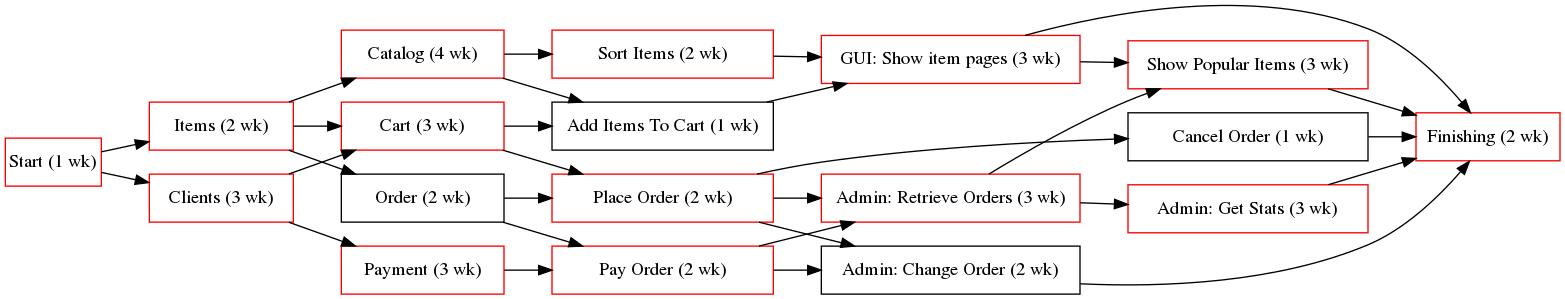
\includegraphics[width=13.5cm]{pert.jpg}
\caption{Gegeven PERT chart van de delen van het project. De kritieke paden zijn aangegeven in het rood.}
\label{pert}
\end{figure}

\begin{figure}
\centering
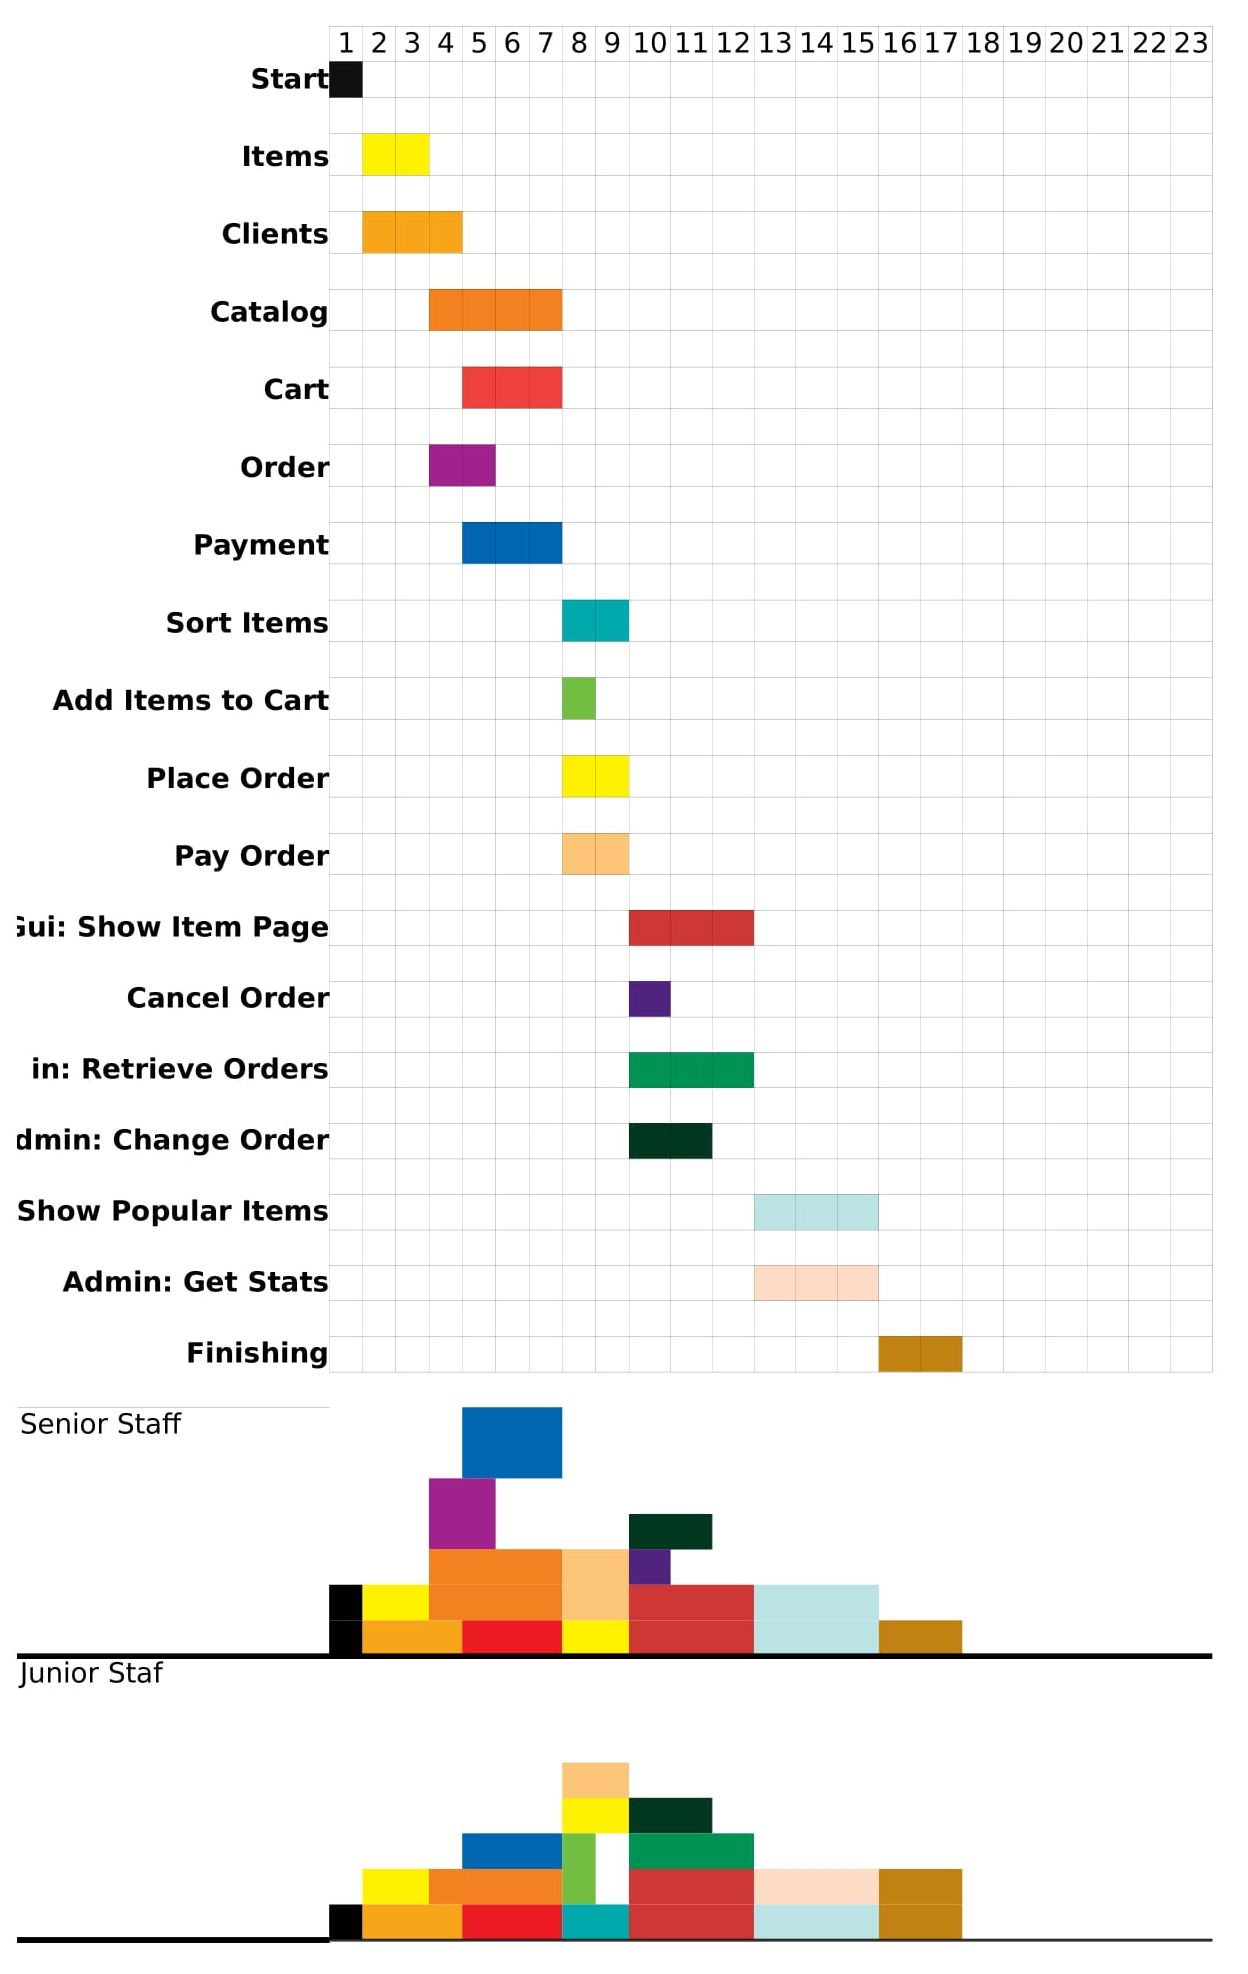
\includegraphics[width=13.5cm]{nolimStaffPlanning.jpg}
\caption{Boven is de Gantt chart te zien waarbij er oneindig veel mankracht gebruikt mag worden. Daaronder is de werkverdeling per week te zien.}
\label{nolimitGantt}
\end{figure}

\begin{figure}
\centering
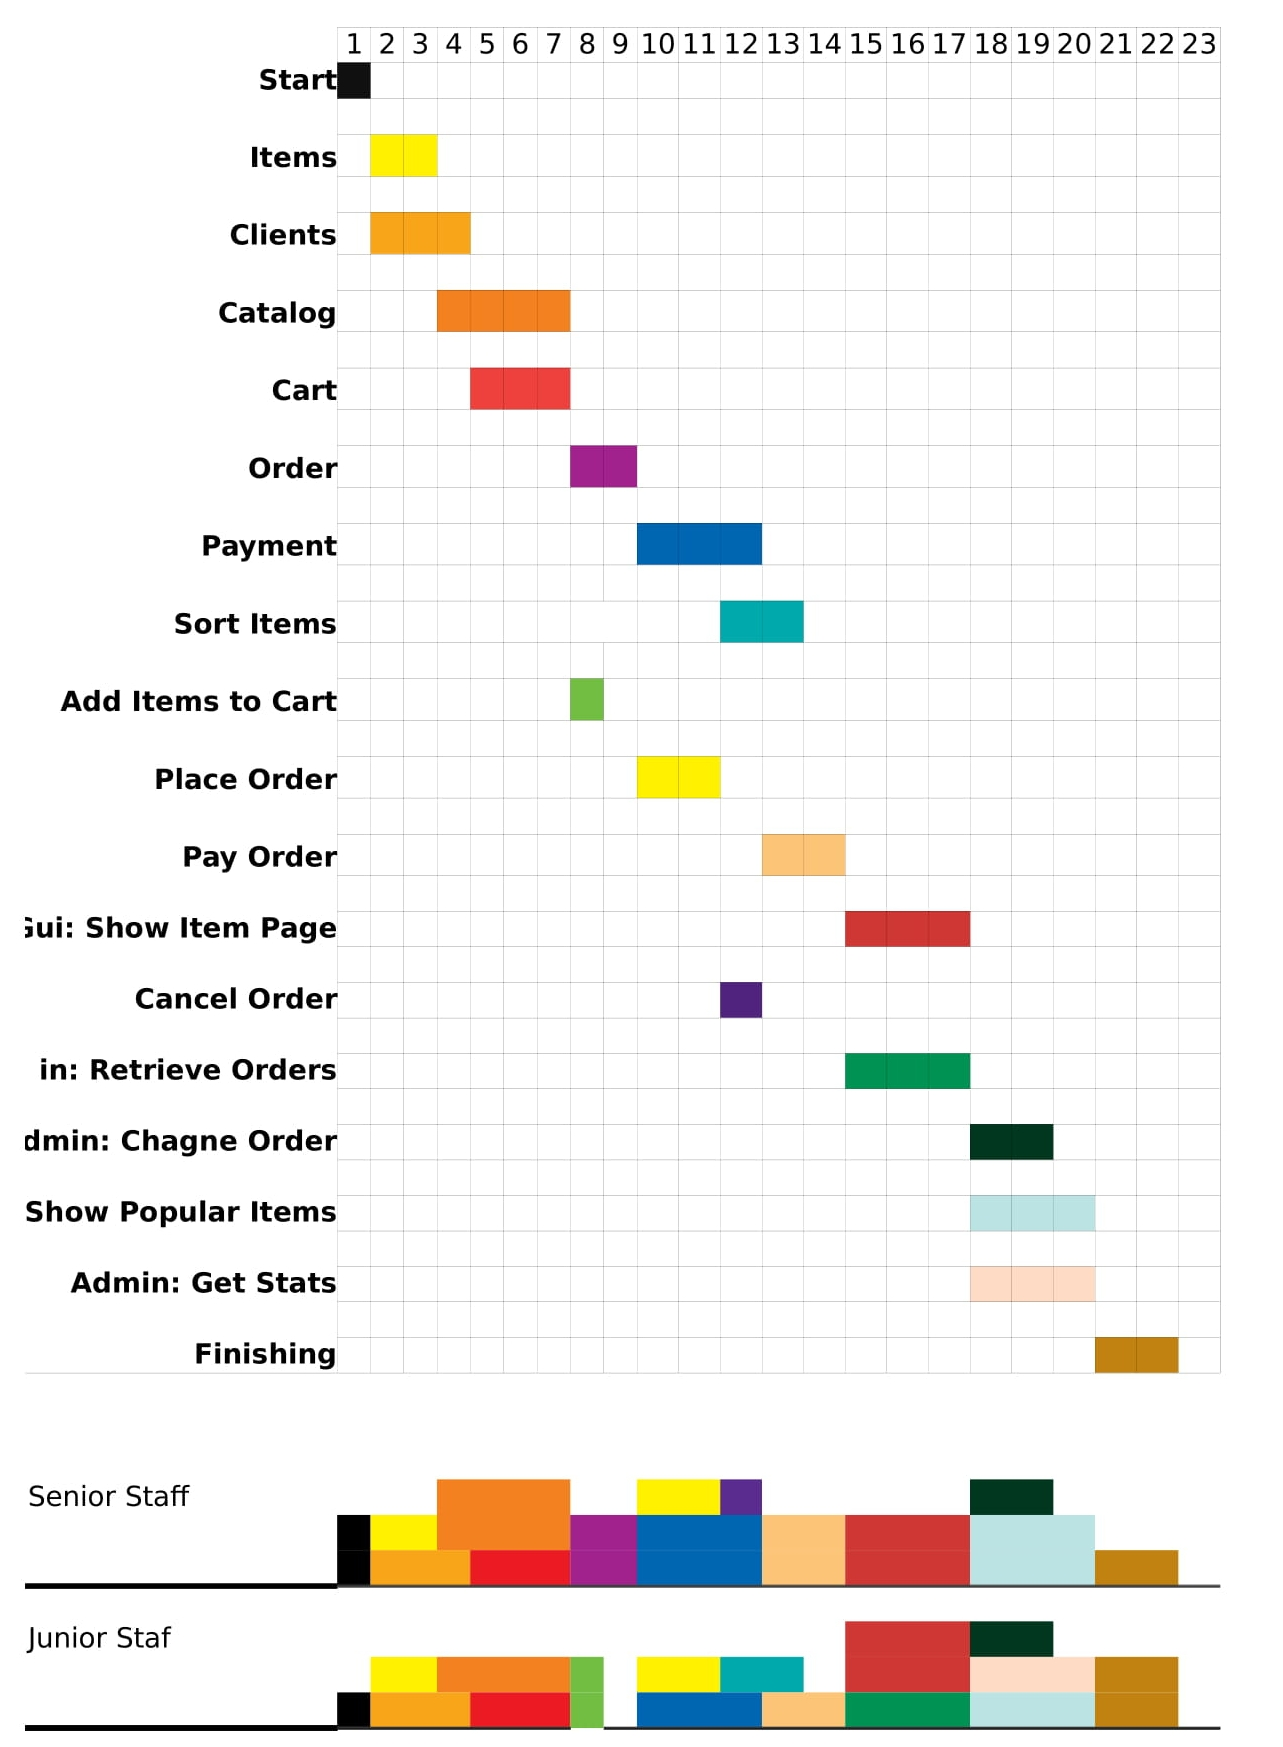
\includegraphics[width=13.5cm]{maxStaffPlanning.jpg}
\caption{Boven is de Gantt chart te zien waarbij er maximaal drie senioren en drie junioren developers ten alle tijde aanwezig zijn. Daaronder is de werkverdeling per week te zien.}
\label{maxGantt}
\end{figure}

\begin{figure}
\centering
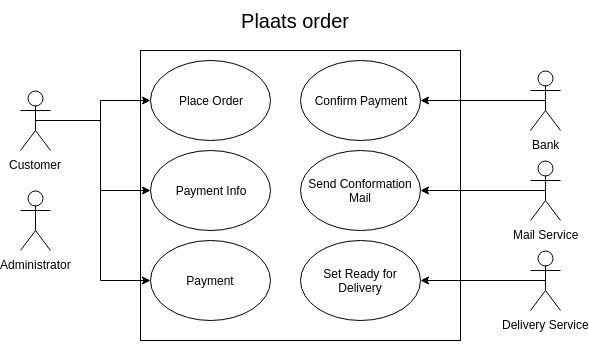
\includegraphics[width=13.5cm]{scenario1_plaatsOrder.jpg}
\caption{Boven is het eerste scenario te zien waarbij er een order wordt geplaatst en betaald.}
\label{scenario1}
\end{figure}
\begin{figure}
\centering
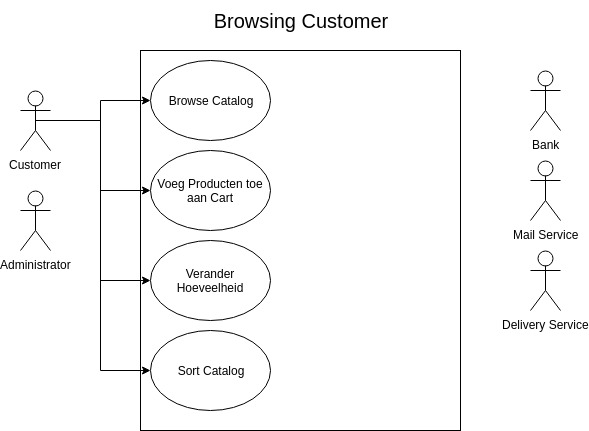
\includegraphics[width=13.5cm]{scenario2_browsingCustomer.jpg}
\caption{Boven is het tweede scenario te zien waarbij een customer aan het zoeken is naar producten.}
\label{scenario2}
\end{figure}
\begin{figure}
\centering
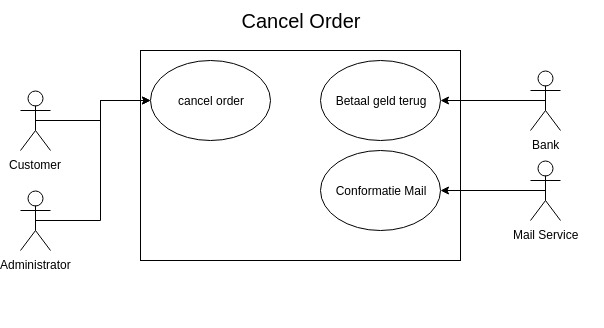
\includegraphics[width=13.5cm]{scenario3_cancelOrderAfterPayment.jpeg}
\caption{Boven is het derde scenario te zien waarbij de customer of de administrator een order cancelled.}
\label{scenario3}
\end{figure}
\begin{figure}
\centering
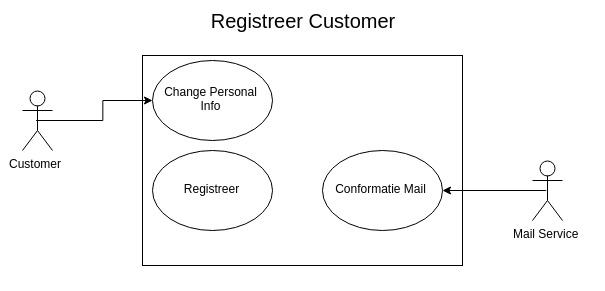
\includegraphics[width=13.5cm]{scenario4_registreer.jpeg}
\caption{Boven is het vierde scenario te zien. Een customer registreert zichzelf hier.}
\label{scenario4}
\end{figure}
\begin{figure}
\centering
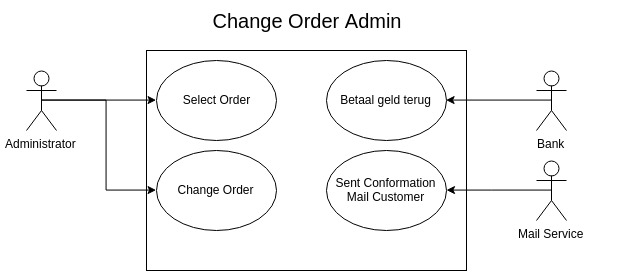
\includegraphics[width=13.5cm]{scenario5.jpg}
\caption{Boven is het vijfde en laatste scenario te zien. Ze laat zien wat er gebeurd als een administrator een order wil veranderen.}
\label{scenario5}
\end{figure}









\begin{table}
\begin{tabular}{|l||l|}
\hline
\multicolumn{2}{|c|}{ Class \textbf{Catalog} }\\ \hline
\multicolumn{2}{|c|}{}\\ \hline
\multicolumn{2}{|c|}{ \textbf{Sub/Super-classes} }\\ \hline
\multicolumn{2}{|c|}{/} \\ \hline
\multicolumn{2}{|c|}{ \textbf{Responsibilities}}\\ \hline
\textbf{Responsibility} & \textbf{Collaboration} \\ \hline
Sort Items By Category & Item \\ \hline
Display To Catalog & Client \\ \hline
\end{tabular}
\begin{tabular}{|l||l|}
\hline
\multicolumn{2}{|c|}{ Class \textbf{User} }\\ \hline
\multicolumn{2}{|c|}{}\\ \hline
\multicolumn{2}{|c|}{ \textbf{Sub/Super-classes} }\\ \hline
\multicolumn{2}{|c|}{Sub: Client} \\ \hline
\multicolumn{2}{|c|}{ \textbf{Responsibilities}}\\ \hline
\textbf{Responsibility} & \textbf{Collaboration} \\ \hline
 &  \\ 
 &  \\
 \hline
\end{tabular}

\begin{tabular}{|l||l|}
\hline
\multicolumn{2}{|c|}{ Class \textbf{Item} }\\ \hline
\multicolumn{2}{|c|}{}\\ \hline
\multicolumn{2}{|c|}{ \textbf{Sub/Super-classes} }\\ \hline
\multicolumn{2}{|c|}{/} \\ \hline
\multicolumn{2}{|c|}{ \textbf{Responsibilities}}\\ \hline
\textbf{Responsibility} & \textbf{Collaboration} \\ \hline
Contains amount in stock &  \\ \hline
Contains basic product information &  \\ \hline
\end{tabular}
\begin{tabular}{|l||l|}
\hline
\multicolumn{2}{|c|}{ Class \textbf{Client} }\\ \hline
\multicolumn{2}{|c|}{}\\ \hline
\multicolumn{2}{|c|}{ \textbf{Sub/Super-classes} }\\ \hline
\multicolumn{2}{|c|}{Super: User} \\ \hline
\multicolumn{2}{|c|}{ \textbf{Responsibilities}}\\ \hline
\textbf{Responsibility} & \textbf{Collaboration} \\ \hline
 &  \\ 
 &  \\ 
 \hline
\end{tabular}
\caption{Scenario A : Display Catalog To User}
\label{scenarioA}
\end{table}



\begin{table}
\begin{tabular}{|l||l|}
\hline
\multicolumn{2}{|c|}{ Class \textbf{Cart} }\\ \hline
\multicolumn{2}{|c|}{}\\ \hline
\multicolumn{2}{|c|}{ \textbf{Sub/Super-classes} }\\ \hline
\multicolumn{2}{|c|}{/} \\ \hline
\multicolumn{2}{|c|}{ \textbf{Responsibilities}}\\ \hline
\textbf{Responsibility} & \textbf{Collaboration} \\ \hline
Contains items, each with an amount & Item \\ \hline
Linked to specific Client & Client \\ \hline
\end{tabular}
\begin{tabular}{|l||l|}
\hline
\multicolumn{2}{|c|}{ Class \textbf{User} }\\ \hline
\multicolumn{2}{|c|}{}\\ \hline
\multicolumn{2}{|c|}{ \textbf{Sub/Super-classes} }\\ \hline
\multicolumn{2}{|c|}{Sub: Client} \\ \hline
\multicolumn{2}{|c|}{ \textbf{Responsibilities}}\\ \hline
\textbf{Responsibility} & \textbf{Collaboration} \\ \hline
 & \\
 &  \\ 
 \hline
\end{tabular}

\begin{tabular}{|l||l|}
\hline
\multicolumn{2}{|c|}{ Class \textbf{Item} }\\ \hline
\multicolumn{2}{|c|}{}\\ \hline
\multicolumn{2}{|c|}{ \textbf{Sub/Super-classes} }\\ \hline
\multicolumn{2}{|c|}{/} \\ \hline
\multicolumn{2}{|c|}{ \textbf{Responsibilities}}\\ \hline
\textbf{Responsibility} & \textbf{Collaboration} \\ \hline
Contains basic product information & / \\ \hline
\end{tabular}
\begin{tabular}{|l||l|}
\hline
\multicolumn{2}{|c|}{ Class \textbf{Client} }\\ \hline
\multicolumn{2}{|c|}{}\\ \hline
\multicolumn{2}{|c|}{ \textbf{Sub/Super-classes} }\\ \hline
\multicolumn{2}{|c|}{Super: User} \\ \hline
\multicolumn{2}{|c|}{ \textbf{Responsibilities}}\\ \hline
\textbf{Responsibility} & \textbf{Collaboration} \\ \hline
Can add an Item to its own Cart & Cart, Item  \\ \hline
\end{tabular}
\caption{Scenario B : Add Item to Cart}
\label{scenarioB}
\end{table}





\begin{table}
\begin{tabular}{|l||l|}
\hline
\multicolumn{2}{|c|}{ Class \textbf{Cart} }\\ \hline
\multicolumn{2}{|c|}{}\\ \hline
\multicolumn{2}{|c|}{ \textbf{Sub/Super-classes} }\\ \hline
\multicolumn{2}{|c|}{/} \\ \hline
\multicolumn{2}{|c|}{ \textbf{Responsibilities}}\\ \hline
\textbf{Responsibility} & \textbf{Collaboration} \\ \hline
Contains items, each with an amount & Item \\ \hline
Linked to specific Client & Client \\ \hline
\end{tabular}
\begin{tabular}{|l||l|}
\hline
\multicolumn{2}{|c|}{ Class \textbf{User} }\\ \hline
\multicolumn{2}{|c|}{}\\ \hline
\multicolumn{2}{|c|}{ \textbf{Sub/Super-classes} }\\ \hline
\multicolumn{2}{|c|}{Sub: Client} \\ \hline
\multicolumn{2}{|c|}{ \textbf{Responsibilities}}\\ \hline
\textbf{Responsibility} & \textbf{Collaboration} \\ \hline
 &  \\ 
 &  \\
 \hline
\end{tabular}

\begin{tabular}{|l||l|}
\hline
\multicolumn{2}{|c|}{ Class \textbf{Item} }\\ \hline
\multicolumn{2}{|c|}{}\\ \hline
\multicolumn{2}{|c|}{ \textbf{Sub/Super-classes} }\\ \hline
\multicolumn{2}{|c|}{/} \\ \hline
\multicolumn{2}{|c|}{ \textbf{Responsibilities}}\\ \hline
\textbf{Responsibility} & \textbf{Collaboration} \\ \hline
Contains basic product information & / \\ \hline
\end{tabular}
\begin{tabular}{|l||l|}
\hline
\multicolumn{2}{|c|}{ Class \textbf{Client} }\\ \hline
\multicolumn{2}{|c|}{}\\ \hline
\multicolumn{2}{|c|}{ \textbf{Sub/Super-classes} }\\ \hline
\multicolumn{2}{|c|}{Super: User} \\ \hline
\multicolumn{2}{|c|}{ \textbf{Responsibilities}}\\ \hline
\textbf{Responsibility} & \textbf{Collaboration} \\ \hline
Can remove an Item to its own Cart & Cart, Item  \\ \hline
\end{tabular}

\caption{Scenario C : Remove Item to Cart}
\label{scenarioC}
\end{table}


\begin{table}
\begin{tabular}{|l||l|}
\hline
\multicolumn{2}{|c|}{ Class \textbf{Item} }\\ \hline
\multicolumn{2}{|c|}{}\\ \hline
\multicolumn{2}{|c|}{ \textbf{Sub/Super-classes} }\\ \hline
\multicolumn{2}{|c|}{/} \\ \hline
\multicolumn{2}{|c|}{ \textbf{Responsibilities}}\\ \hline
\textbf{Responsibility} & \textbf{Collaboration} \\ \hline
Contains basic product information & / \\ \hline
\end{tabular}
\begin{tabular}{|l||l|}
\hline
\multicolumn{2}{|c|}{ Class \textbf{Client} }\\ \hline
\multicolumn{2}{|c|}{}\\ \hline
\multicolumn{2}{|c|}{ \textbf{Sub/Super-classes} }\\ \hline
\multicolumn{2}{|c|}{Super: User} \\ \hline
\multicolumn{2}{|c|}{ \textbf{Responsibilities}}\\ \hline
\textbf{Responsibility} & \textbf{Collaboration} \\ \hline
 & \\ \hline
\end{tabular}

\begin{tabular}{|l||l|}
\hline
\multicolumn{2}{|c|}{ Class \textbf{User} }\\ \hline
\multicolumn{2}{|c|}{}\\ \hline
\multicolumn{2}{|c|}{ \textbf{Sub/Super-classes} }\\ \hline
\multicolumn{2}{|c|}{Sub: Administrator, Client} \\ \hline
\multicolumn{2}{|c|}{ \textbf{Responsibilities}}\\ \hline
\textbf{Responsibility} & \textbf{Collaboration} \\ \hline
 &  \\ \hline
\end{tabular}
\begin{tabular}{|l||l|}
\hline
\multicolumn{2}{|c|}{ Class \textbf{Administrator} }\\ \hline
\multicolumn{2}{|c|}{}\\ \hline
\multicolumn{2}{|c|}{ \textbf{Sub/Super-classes} }\\ \hline
\multicolumn{2}{|c|}{Super: User} \\ \hline
\multicolumn{2}{|c|}{ \textbf{Responsibilities}}\\ \hline
\textbf{Responsibility} & \textbf{Collaboration} \\ \hline
Can change orders & Order  \\ \hline
\end{tabular}

\begin{tabular}{|l||l|}
\hline
\multicolumn{2}{|c|}{ Class \textbf{Order} }\\ \hline
\multicolumn{2}{|c|}{}\\ \hline
\multicolumn{2}{|c|}{ \textbf{Sub/Super-classes} }\\ \hline
\multicolumn{2}{|c|}{/} \\ \hline
\multicolumn{2}{|c|}{ \textbf{Responsibilities}}\\ \hline
\textbf{Responsibility} & \textbf{Collaboration} \\ \hline
Contains items, each with an amount & Item \\ \hline
Linked to specific Client & Client \\ \hline
Has an order ID & / \\ \hline
Has a flag 'delivered' & / \\ \hline
\end{tabular}

\caption{Scenario D : Admin changes order}
\label{scenarioD}
\end{table}

\begin{table}
\begin{tabular}{|l||l|}
\hline
\multicolumn{2}{|c|}{ Class \textbf{Item} }\\ \hline
\multicolumn{2}{|c|}{}\\ \hline
\multicolumn{2}{|c|}{ \textbf{Sub/Super-classes} }\\ \hline
\multicolumn{2}{|c|}{/} \\ \hline
\multicolumn{2}{|c|}{ \textbf{Responsibilities}}\\ \hline
\textbf{Responsibility} & \textbf{Collaboration} \\ \hline
Contains basic product information & / \\ \hline
\end{tabular}

\begin{tabular}{|l||l|}
\hline
\multicolumn{2}{|c|}{ Class \textbf{Order} }\\ \hline
\multicolumn{2}{|c|}{}\\ \hline
\multicolumn{2}{|c|}{ \textbf{Sub/Super-classes} }\\ \hline
\multicolumn{2}{|c|}{/} \\ \hline
\multicolumn{2}{|c|}{ \textbf{Responsibilities}}\\ \hline
\textbf{Responsibility} & \textbf{Collaboration} \\ \hline
Contains items, each with an amount & Item \\ \hline
Linked to specific Client & Client \\ \hline
Calculates a total price based on Items & Item \\ \hline
Has an order ID & / \\ \hline
Has a flag 'Paid' & / \\ \hline
\end{tabular}

\begin{tabular}{|l||l|}
\hline
\multicolumn{2}{|c|}{ Class \textbf{Cart} }\\ \hline
\multicolumn{2}{|c|}{}\\ \hline
\multicolumn{2}{|c|}{ \textbf{Sub/Super-classes} }\\ \hline
\multicolumn{2}{|c|}{/} \\ \hline
\multicolumn{2}{|c|}{ \textbf{Responsibilities}}\\ \hline
\textbf{Responsibility} & \textbf{Collaboration} \\ \hline
Contains items, each with an amount & Item \\ \hline
Linked to specific Client & Client \\ \hline
Checkout to Order & Item, Client, Order \\ \hline
\end{tabular}

\begin{tabular}{|l||l|}
\hline
\multicolumn{2}{|c|}{ Class \textbf{User} }\\ \hline
\multicolumn{2}{|c|}{}\\ \hline
\multicolumn{2}{|c|}{ \textbf{Sub/Super-classes} }\\ \hline
\multicolumn{2}{|c|}{Sub: Client} \\ \hline
\multicolumn{2}{|c|}{ \textbf{Responsibilities}}\\ \hline
\textbf{Responsibility} & \textbf{Collaboration} \\ \hline
 &  \\ \hline
\end{tabular}
\begin{tabular}{|l||l|}
\hline
\multicolumn{2}{|c|}{ Class \textbf{Client} }\\ \hline
\multicolumn{2}{|c|}{}\\ \hline
\multicolumn{2}{|c|}{ \textbf{Sub/Super-classes} }\\ \hline
\multicolumn{2}{|c|}{Super: User} \\ \hline
\multicolumn{2}{|c|}{ \textbf{Responsibilities}}\\ \hline
\textbf{Responsibility} & \textbf{Collaboration} \\ \hline
 & \\ \hline
\end{tabular}
\caption{Scenario E : Place Order and Pay}
\label{scenarioE}
\end{table}



\end{document}